\begin{figure*}[htbp]
\centering
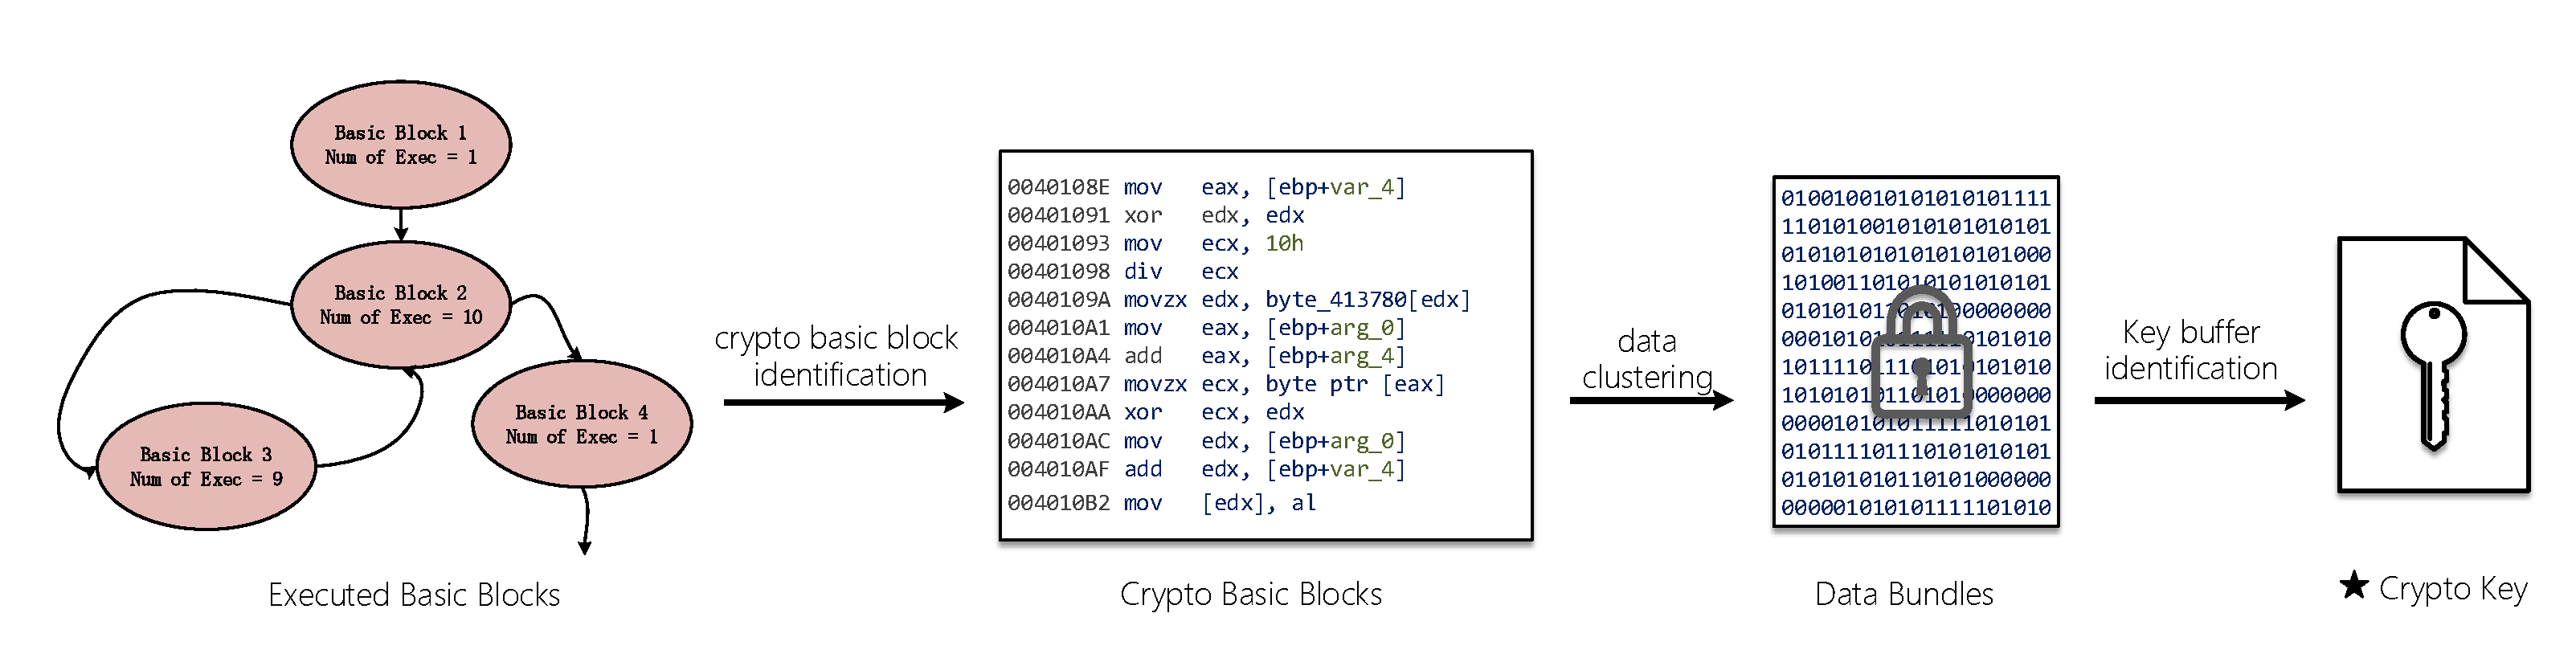
\includegraphics[width=\textwidth]{keyPinpoint.pdf}
\caption{The process of pinpointing crypto keys in binary executables\label{fig:cry} }
\end{figure*}

%An overview of \sysname is presented in~\autoref{fig:workflow}. 
\sysname uses dynamic analysis to identify insecure crypto keys. 
It assumes that there exist test cases to execute the program so that it uses the crypto operations. Our approach uses dynamic analysis because it needs statistics about the program execution.
%  randomness of the runtime data, and also the number of executions of basic blocks. 
Furthermore, static analysis faces many limitations for analyzing memory buffers, which store the crypto keys.
%
At a high level, \sysname comprises of two phases:

\begin{compactitem}

\item \textbf{Pinpointing the Key}. 
In the first phase, detailed in~\S\ref{sec:analysis:pinpoint}, the target program is executed with a lightweight coarse-grained  binary code instrumentation to firstly identify the crypto basic blocks and then identify the crypto keys they use.

\item \textbf{Detecting the Insecure Key}. In the second phase, detailed in~\S\ref{sec:analysis:misuse}, the target program is executed again with a heavyweight  fine-grained  instrumentation, which tracks the memory reads and writes and conducts a function level taint analysis. 
% with the user or system generated input. 
Through taint analysis of the pinpointed keys, \sysname then detects the insecure crypto keys. \looseness=-1

\end{compactitem}


\subsection{Pinpointing Crypto Keys}\label{sec:analysis:pinpoint}

The first phase of \sysname is to pinpoint the crypto keys. 
An overview of how \sysname performs this analysis is presented in~\autoref{fig:cry}. 
%We define a crypto operation as the set of crypto basic blocks executed during a specific application (e.g., an HTTPS communication).
It first identifies the crypto basic blocks by running the executable with multiple test inputs, and then analyzes the data those basic blocks operate on to locate the crypto keys. 
% Consequently, this analysis consists of two steps: (i) crypto basic block identification, and (ii) crypto key buffer identification.

\paragraph{Step-I: Crypto {Basic Block} Identification} % \label{sec:analysis:pinpoint:locate}
One observation of modern crypto algorithms (e.g., \textsf{\small AES}, \textsf{\small RSA},  \textsf{\small DSA}) is that they are typically built with only a few compact transformations, which correspond to just a few basic blocks in a program. 
Therefore, if we can identify these basic blocks, we would  identify the crypto operations that use them. 
% To achieve this, we leverage a number of common features to identify a crypto basic block. 

\begin{Definition}
\label{def:cryptoblock}
A crypto basic block is defined as a basic block that satisfies the following constraints: 
(i) the basic block uses arithmetic calculations to implement a cryptographic  operation; 
(ii) the basic block is executed multiple times to mix a data stream with a key stream; 
%(iii) the produced (or consumed) data should have both high entropy and high randomness.
(iii) the produced or consumed data have high randomness.
% that reflect strong cryptographic features such as frequently using arithmetic instructions and producing highly random data.
\end{Definition}

Our approach first computes, for each basic block, the ratio of  x86/64 arithmetic and bitwise instructions (e.g., \texttt{mul}, and \texttt{xor})~\cite{caballero2009dispatcher, intelx86}. 
A basic block is considered a candidate crypto basic block if it has a ratio larger than a pre-defined threshold. 
This threshold has been experimentally selected as 15\% in our current design after analyzing common crypto libraries and utilities.
A special case is that a basic block is directly considered a candidate if it contains instructions from the Advanced Encryption Standard instruction set (AES-NI),  an extension to the x86 instruction set for microprocessors from Intel and AMD.

Next, it checks whether the candidate basic blocks are \emph{data sensitive}. 
A basic block is data sensitive if the total amount of execution for the basic block is proportional to the size of its input data. 
We prepare four test suites with inputs of different size magnitude to test the program, and calculate for each candidate basic block, 
the total number of executions of the basic block across all inputs, the total basic block's input data size, and the total basic block's output data size. 
Candidate basic blocks for which the number of executions increases approximately linearly with the ratio of input/output data size are kept as candidate crypto basic blocks. Other candidates are discarded.
 
At this point, our approach has checked the first two conditions  in Definition~\ref{def:cryptoblock}. 
The last condition checks if the data operated on by the candidate basic block has high randomness. 
However, each time a basic block is executed it only operates on part of the input data. 
Thus, our approach accumulates all the data that each candidate basic block operates on during the entire program execution into data bundles.

\begin{Definition}
A data bundle is defined as the sequence of all the data that an operand of an instruction operates on during the entire execution of the program. The size of a data bundle is the number of data items it contains.
\end{Definition}

{For example, in Figure~\ref{fig:dd:asm} the instruction at \texttt{0x0040109A} has one memory read operation and is executed 256 times. Therefore, there will be a data bundle with 256 data items: the sequence of value read that is from \texttt{byte\_413780[edx]}.
% and the sequence of value write that is to \texttt{edx}.} \ZQ{not clear to me. Since this is written to register edx, why there is a bundle?}
%
Our approach focuses on data bundles that are generated by  instructions with memory operands, since registers have a limited size that does not typically hold a crypto key.
%We search for high entropy data among all data bundles. 
Once the data bundles are built, they are examined to identify those that contain highly random data. 
%Interestingly, many other data transformations (especially data compression) could also generate data of high entropy. 
%Hence, we should further distinguish crypto operations from other data encoding operations. 
%Fortunately, while data encoding operation may generate data of high entropy, the randomness of crypto data is actually distinguishable~\cite{wang2013steal}. 
%From this point of view, if a bundle has high-entropy, it is checked using an in-depth data randomness analysis with \emph{Chi-Square distribution} and \emph{Monte Carlo} $\pi$ \emph{approximation} tests. 
For this, {our approach leverages the \textsf{\small ent}~\cite{ent_random} utility to measure the randomness of the collected data bundle with both \emph{Chi-Square distribution} and \emph{Monte Carlo} $\pi$ \emph{approximation} tests}.
If \textsf{\small ent} judges the data bundle as random, the candidate basic block is considered a crypto basic block.

In our running example in Figure~\ref{fig:dd:asm}, the basic block (\texttt{0x0040108E}-\texttt{0x004010B2}) is the crypto basic block to be identified.
It satisfies the above constraints for a crypto basic block:
	it utilizes arithmetic and bitwise instructions to implement the crypto operation, 
	the number of executions of the basic block is proportional to the size of the input data, 
	it accesses several memory buffers, and its produced data has high randomness.

\paragraph{Step-II: Crypto Key Buffer Identification}
Having identified the crypto basic blocks in Step-I, our approach next identifies the crypto keys used by those basic blocks. 
Different types of data may be handled by a crypto basic block: crypto key, plaintext, ciphertext, and message to be signed. 
More concretely, a crypto operation will take two inputs: 
crypto key and plaintext for encryption, 
crypto key and ciphertext for decryption, and 
crypto key and message for digital signature. 
Thus, the crypto key should always be an input to the crypto basic block. 
Therefore, we can exclude the data output by the crypto basic block and just focus on the input data. 
Still, our approach has to separate the crypto key from the other input. 
And, it  can no longer use randomness for this since both the crypto key and the ciphertext will have high randomness.

\begin{Definition}
A crypto buffer is defined as all operated memory addresses in one data bundle of a crypto basic block,
and the size of a crypto buffer is the number of unique memory addresses it contains. 
\end{Definition}

{For instance, the memory read data bundle of the  instruction at \texttt{0x0040109A} in Figure~\ref{fig:dd:asm} contains 256 items.
This bundle, however, only contains 16 unique memory addresses, thus the size of corresponding crypto buffer is 16 instead of 256.
When we test the randomness of the data, we use the concept of bundle because a buffer may be accessed randomly and we should concern about the access sequence.
If the high randomness is discovered, we then only concern about the range of accessed memory,
	and thus we use the concept of buffer to help distinguish key from data.
}

To identify which input is the crypto key buffer, \sysname leverages the following two complementary insights.

\begin{compactitem}
\item \textbf{Using the buffer size}. 
Typically, the crypto key buffer is small compared to the ciphertext/plaintext/message buffer: a key can be stored in a relatively small buffer but the crypto input often needs a larger memory buffer. 
This feature becomes even more obvious when executing the crypto basic blocks with multiple inputs: either the key is repeatedly used or it is updated between different iterations (e.g., the state update of a stream cipher), and the key is generally stored in a fixed-length memory buffer whereas the length of the ciphertext/plaintext/message varies according to the size of the program input.
% Please note that we can test the program with inputs of different sizes, or execute the program repeatedly  to observe the variation of the input buffer, and exclude those non-key buffers.}

\item \textbf{Using the execution context}.
The other insight is that crypto keys and other input data are typically initialized by different functions. 
If we track the execution context of how the data is initialized, we can easily differentiate them as well. 
For instance, the used crypto key buffer is usually initialized by a key derivation function or from a pseudo-random number generator, while the plaintext/ciphertext/message is generally directly read from a file or network socket. 

\end{compactitem}


\subsection{Detecting Insecure Keys}
\label{sec:analysis:misuse}

The second phase of \sysname detects the insecure crypto keys. 
Unlike the first phase where we perform a lightweight dynamic binary analysis to collect execution statistics (e.g., the number of executions for a basic block and the randomness of data bundles), the second phase requires a heavyweight dynamic binary analysis to trace how keys are generated and propagated.
At a high level, our analysis is a function-level variant of dynamic taint analysis (e.g,.~\cite{song2005ndss, schwartz2010oakland}) with the following taint policies. \looseness=-1

\paragraph{Taint Sources} 
\sysname uses three different taint tags to capture whether a value has been derived from a local input  (i.e., filesystem or return value from the \texttt{rand} function), a remote input (i.e., the network), or 
none of those two (i.e., deterministic value). 
Thus,  each memory location (i.e., byte) in the shadow memory~\cite{schwartz2010oakland} has a two-bit taint tag with values 00 for no input, 01 for local input, and 10 for remote input.  
At initialization, all memory locations will be assigned the no-input tag. 
During program execution, if \sysname observes that a memory location is assigned from local input (remote input), \sysname assigns the local (remote) taint tag to the memory location. 
For instance, \texttt{Key} at line 13 in our running example in Figure~\ref{fig:dd:code} will be assigned with a local input tag. 


In addition, to quantitatively measure how many of bytes of information generated for crypto keys, we introduce the concept of the length of input for the buffer involved for key generation.
\begin{Definition}
The input length (IL) of a buffer is the number of bytes derived from program inputs.
\end{Definition}
\noindent
For instance, in our running example the \texttt{keygen} function initializes four bytes of the \texttt{seed} buffer using function \texttt{rand}. Then \sysname keeps a 4-byte IL for this buffer.


\paragraph{Taint Propagation} \sysname could use a fine-grained taint analysis (e.g.,~\cite{song2005ndss}) to trace each instruction and propagate the taint tags correspondingly. 
However, we found such an approach often incurs high performance overhead to the analyzed program, e.g., causing a remote peer to close the network socket due to connection time out, or the GUI freezing for non-networking programs, e.g., \textsf{\small WinRAR}. 
Therefore, we have develop a lightweight, function-level, taint propagation policy, which propagates  taint tags based only on the memory read and memory write operations inside the execution context of a function.
This propagation is based on the fact that \sysname only requires knowing whether a buffer contains data from either deterministic, local input, or remote input (i.e., the three taint tags). 
Therefore, it does not need to propagate the taint tags precisely for each instruction. 
Instead, it can propagate taint tags at the higher function level, significantly improving efficiency.

More specifically, \sysname taints all the data definitions (i.e., memory writes) inside a function using the taint tag of the input data. 
% (i.e., determined by the memory read instructions) to this function. 
As such, it only needs to instrument the memory read and write instructions. 
The memory read instructions define the taint source for the function, and the memory write instructions define the taint tags for the memory data based on the current function's taint . 
If a new taint source to the function is observed, the new taint tags are unioned with the current function's taint tag. All the defined data inside this function will from that point on have a unioned taint tag (e.g., tag with bits 11 to represent both local and remote input). 
In our running example, the \texttt{seed} buffer in the \texttt{keygen} function  will be tainted with local input tag, and thus the global \texttt{Key} buffer will also be assigned the local input tag. 
% Note that the reason of why we are only concerned with memory data (register data is not included) is because crypto keys usually have a larger length (e.g., at least 128 or 256 bits, etc.) and typically cannot be hold by registers. 




%\review{In addition, to quantitatively measure the randomness of the information contained in a buffer, we define the IL of a buffer as the bytes directly derived from program inputs or indirectly transferred from other buffers.
%For instance, in our running example the \texttt{keygen} function initializes four bytes of the \texttt{seed} buffer using \texttt{rand}. Then \sysname keeps a 4-byte IL for this buffer.
%}

{
While propagating the taint tags, we also propagate the IL for the buffers. Such information is particularly useful for determining whether a key has sufficient randomness. In particular, for each function, \sysname tracks the total number of IL. Then whenever there is a memory write information, it propagates the current IL to this buffer. When the function returns, it recalculates the IL for each buffer based on both the number of bytes accessed and also the current IL for this function. 
% If a buffer is not directly initialized by the program input, \sysname assigns an IL to it according to all accessed intermediate buffers in a function.
% To implement this, \sysname keeps tracking the buffer accessed by one function as soon as it starts executing. 
Assume that one function accesses two buffers during its execution.
\sysname records how many bytes in each buffer are accessed, respectively.
If the number of bytes does not exceed the IL of the host buffer,
	\sysname adds this number to the IL of the newly initialized buffer.
Otherwise it adds the IL of the host buffer to the IL of the new buffer.
Finally, we check whether the IL of the new buffer is larger than the size of the buffer.
If so, the IL is adjusted to the size of the buffer.
Through performing such IL propagation, \sysname maps the information from input buffer to the output buffer of one function.
 }

% \ZQ{shall this paragraph go to the taint source? when we taint the source of input, we also track the input length when we see such input?}

% \ZQ{In the taint propagation, we need to track the size of input length for a buffer.}


\paragraph{Taint Sinks} With the aforementioned taint sources and taint propagation policy, all the memory locations will have a taint tag showing whether the data comes from local or remote input, or is deterministic. 
To identify insecure crypto keys, 
\sysname checks the taint tag of the buffer at the crypto basic block (to check whether the key is improperly generated) or when the program exits (to check for key residue). 
In particular, we use the following policies to detect the insecure crypto keys.

\begin{compactitem}
\item \textbf{Detecting DGK}. 
If a key is not derived from any input, i.e., is deterministic,  
then \sysname considers that the generation of the key is flawed.
{
In addition, \sysname checks whether the key receives enough information from non-deterministic inputs.
This is done through an analysis of the key buffer IL.
For example, in our running example the key is initialized in the \texttt{keygen} function.
At the beginning of the function a \texttt{seed} buffer is initialized with a 4-byte IL.
Then the \texttt{key} buffer in the same function is initialized.
At that time, the IL of the \texttt{key} buffer is also assigned as 4 because the function only accesses one buffer with a 4-byte IL.
As a result, even if the size of the \texttt{key} buffer is 16, it has a smaller IL of 4-byte.
Eventually, if the IL of a key buffer has the size less than a threshold, 16 bytes (128 bits) in our current design, we consider the key is insecure.
In this case the used key buffer has a 4-byte IL and is obviously insecure.
}

% In our running example, the length of the key is actually 16 bytes, which will be detected insecure by \sysname.

%\ZQ{it is not clear how the length of the IL is computed. What do you mean the sum of these two IL? What do you mean the actual size? Maybe give an example}

%\JR{The example is provided, and since the size of used key in our running example equals to 16 bytes, we do not consider it an insecure one.}

\item \textbf{Detecting INK}. 
An insecurely negotiated key is a crypto key shared between two parties (e.g., a session key between a client and a server) where the key value is only influenced by one party~\cite{keyValidated2017}. 
{A negotiated key is the symmetric key used for encrypting or decrypting network data.}
If we know there is a negotiated key but the taint tag for this key includes only local input tag or remote input tag (not both), \sysname considers this is an insecurely negotiated key. \looseness=-1

\item \textbf{Detecting RK}. 
When a crypto operation terminates, all memory buffers holding involved crypto keys should be cleared~\cite{yang2017dead}. 
%Since we have located the keys and tracked their propagation (even though this is at a coarse granularity), 
To detect any recoverable keys, 
\sysname searches the memory to check any partial existences of the keys in memory 
when the process terminates. 
A key is considered recoverable if one third of its content still exists in memory~\cite{heninger2009reconstructing}. 
Therefore, we cross check the content of the data bundles, and if one third of the content still matches with the original key buffer, \sysname considers it a recoverable key. 
{In our running example, the \texttt{Key} buffer is allocated in the global memory region, and is not cleared after process termination. \sysname therefore detects it is an RK case.}

\end{compactitem}


